\documentclass{beamer}
\usepackage{beamerthemesplit}
\usepackage{wrapfig}
\usetheme{SPbGU}
\usepackage{pdfpages}
\usepackage{amsmath}
\usepackage{cmap} 
\usepackage[T2A]{fontenc} 
\usepackage[utf8]{inputenc}
\usepackage[english,russian]{babel}
\usepackage{indentfirst}
\usepackage{amsmath}
\usepackage{tikz}
\usepackage{multirow}
\usepackage[noend]{algpseudocode}
\usepackage{algorithm}
\usepackage{algorithmicx}
\usetikzlibrary{shapes,arrows}
\usepackage{fancyvrb}

\usepackage{graphicx}
\usepackage[utf8]{inputenc}  
\usepackage{amsmath}
\usepackage{amssymb}
\usepackage{amsthm}
\usepackage{latexsym}
\usepackage{float}
\usepackage{tabularx}
\usepackage{booktabs}

\allowdisplaybreaks

\newtheorem{rutheorem}{Теорема}
\newtheorem{ruproof}{Доказательство}
\newtheorem{rudefinition}{Определение}
\newtheorem{rulemma}{Лемма}

\beamertemplatenavigationsymbolsempty

\title[]{Левая рекурсия в PEG}
\subtitle[]{}
% То, что в квадратных скобках, отображается в левом нижнем углу. 
\institute[]{
Лаборатория языковых инструментов JetBrains \\
Санкт-Петербургский государственный университет \\
Математико-механический факультет }

% То, что в квадратных скобках, отображается в левом нижнем углу.
\author[Екатерина Вербицкая]{Екатерина Вербицкая}

\date{23 ноября 2015г.}

\definecolor{orange}{RGB}{179,36,31}

\begin{document}
{
\begin{frame}[fragile]
  \titlepage
\end{frame}
}

\begin{frame}[fragile]
  \transwipe[direction=90]
  \frametitle{Parser Expression Grammars}
\begin{itemize}
  \item PEG G --- четверка $(V, T, P, p_S)$, где 
    \begin{itemize}
      \item $V$ --- конечное множество нетерминалов
      \item $T$ --- алфавит (конечное множество терминалов) 
      \item $P$ --- функция из $V$ в выражения (parser expression) 
      \item $p_S$ --- стартовое выражение
    \end{itemize}
\end{itemize}
\begin{itemize}
  \item Parser expression
  \begin{itemize}
    \item Пустая строка $\varepsilon$
    \item Терминал $a$
    \item Нетерминал $A$
    \item Последовательность $p_1 p_2$, где $p_1, p_2$ --- parser expression
    \item Упорядоченный выбор $p_1 / p_2$, где $p_1, p_2$ --- parser expression
    \item 0-или-больше $p^*$, где $p$ --- parser expression
    \item Предикат Не $!p$, где $p$ --- parser expression
  \end{itemize}
\end{itemize}
\end{frame}

\begin{frame}[fragile]
  \transwipe[direction=90]
  \frametitle{Отношение PEG}
\begin{center}
  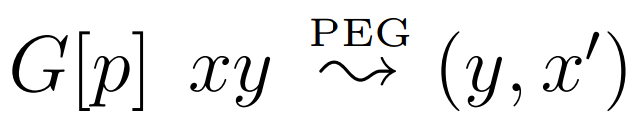
\includegraphics[width=0.3\textwidth]{pics/pegRel}
\end{center}                                      
\begin{itemize}
  \item Выражение \textit{p} парсит строку \textit{xy}, съедая \textit{x} и оставляя \textit{y}, возвращая 
\textit{x'} как результат
  \item Если справа \textit{fail}, значит, распарсить строку не удалось
\end{itemize}
\end{frame}

\begin{frame}[fragile]
  \transwipe[direction=90]
  \frametitle{Операционная семантика PEG: пустая строка}
\begin{center}
  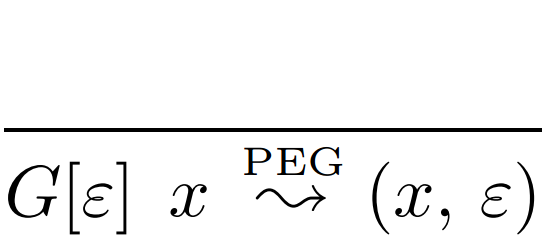
\includegraphics[width=0.3\textwidth]{pics/empty}
\end{center}                                      
\end{frame}

\begin{frame}[fragile]
  \transwipe[direction=90]
  \frametitle{Операционная семантика PEG: терминал}
\begin{center}
  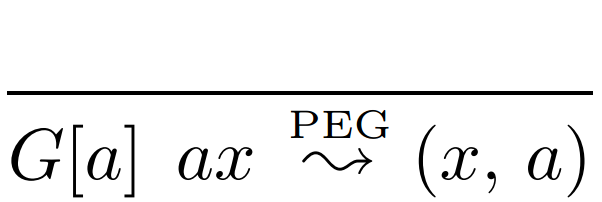
\includegraphics[width=0.35\textwidth]{pics/char1}  \\~\\   \pause
  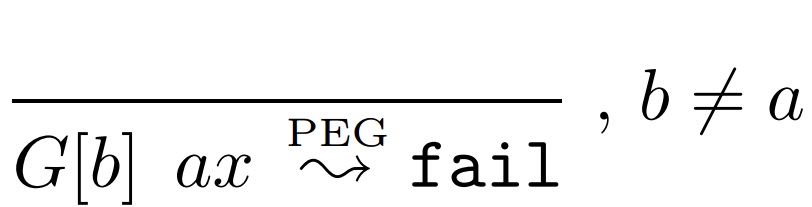
\includegraphics[width=0.5\textwidth]{pics/char2}   \\~\\   \pause
  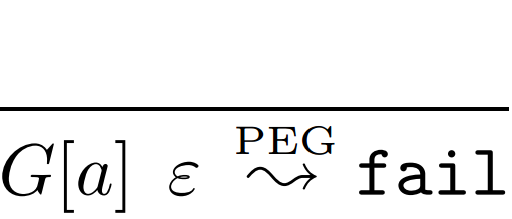
\includegraphics[width=0.3\textwidth]{pics/char3}
\end{center}  
\end{frame}

\begin{frame}[fragile]
  \transwipe[direction=90]
  \frametitle{Операционная семантика PEG: переменная}
\begin{center}
  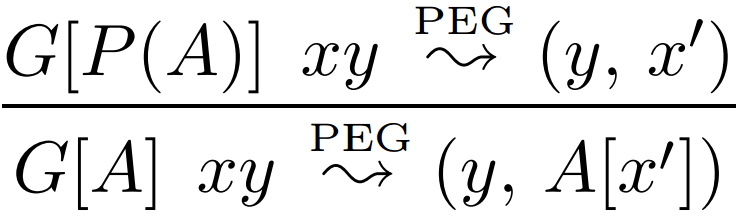
\includegraphics[width=0.4\textwidth]{pics/var1}  \\~\\     \pause
  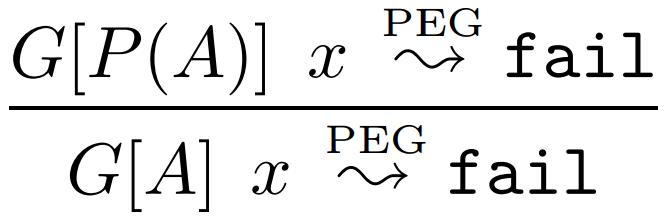
\includegraphics[width=0.35\textwidth]{pics/var2} 
\end{center}
\end{frame}


\begin{frame}[fragile]
  \transwipe[direction=90]
  \frametitle{Операционная семантика PEG: последовательность}
\begin{center}
  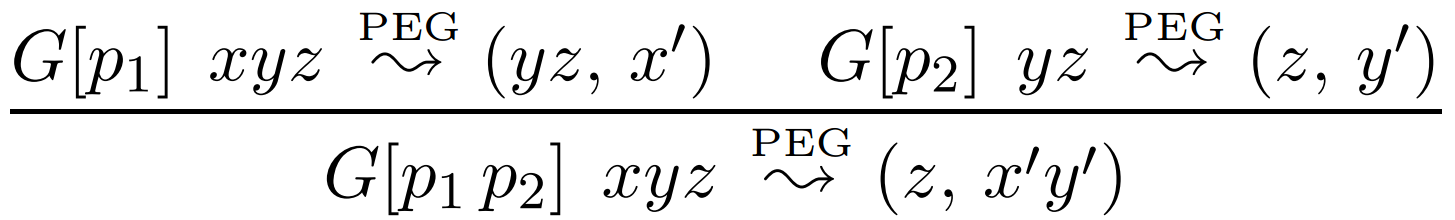
\includegraphics[width=0.7\textwidth]{pics/con1}  \\~\\     \pause
  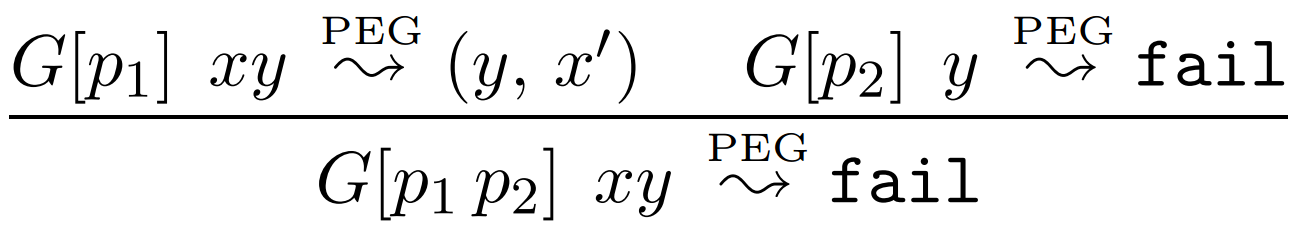
\includegraphics[width=0.7\textwidth]{pics/con2}  \\~\\     \pause
  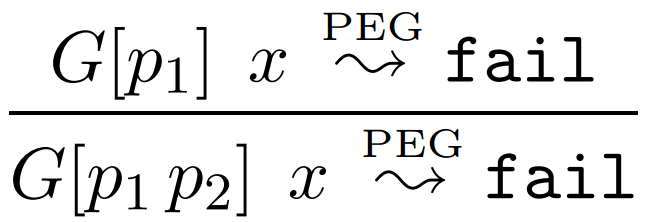
\includegraphics[width=0.35\textwidth]{pics/con3}
\end{center}
\end{frame}

\begin{frame}[fragile]
  \transwipe[direction=90]
  \frametitle{Операционная семантика PEG: выбор}
\begin{center}
  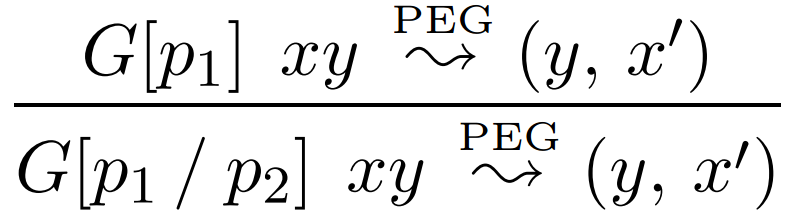
\includegraphics[width=0.4\textwidth]{pics/ord1}  \\~\\     \pause
  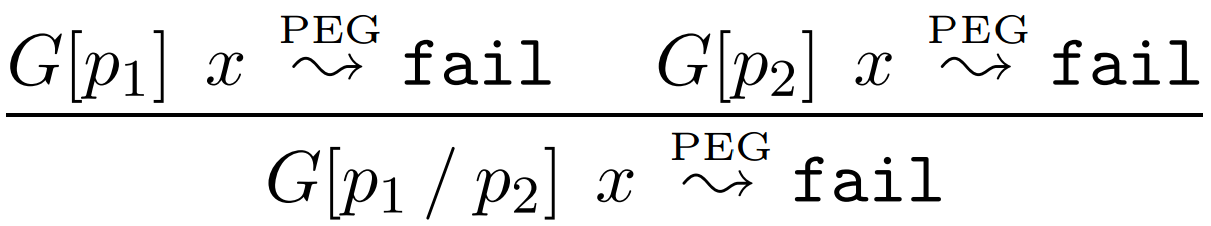
\includegraphics[width=0.6\textwidth]{pics/ord2}  \\~\\     \pause
  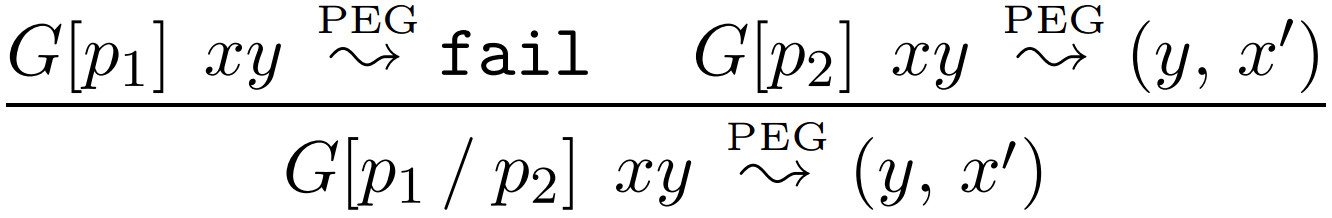
\includegraphics[width=0.65\textwidth]{pics/ord3}
\end{center}
\end{frame}

\begin{frame}[fragile]
  \transwipe[direction=90]
  \frametitle{Операционная семантика PEG: предикат не}
\begin{center}
  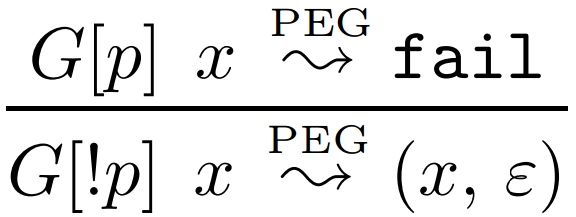
\includegraphics[width=0.3\textwidth]{pics/not1}  \\~\\     \pause
  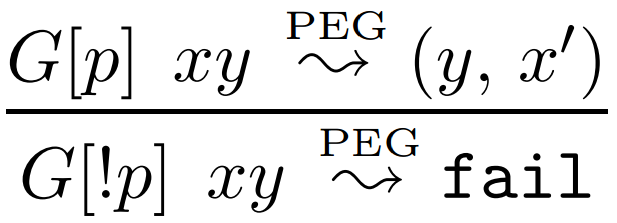
\includegraphics[width=0.35\textwidth]{pics/not2} 
\end{center}
\end{frame}

\begin{frame}[fragile]
  \transwipe[direction=90]
  \frametitle{Операционная семантика PEG: повторение}
\begin{center}
  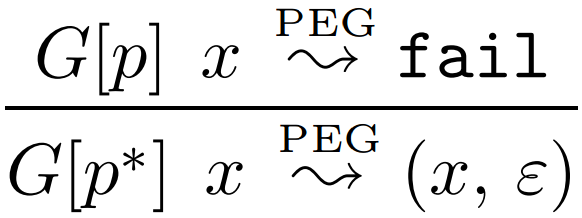
\includegraphics[width=0.3\textwidth]{pics/rep1}  \\~\\     \pause
  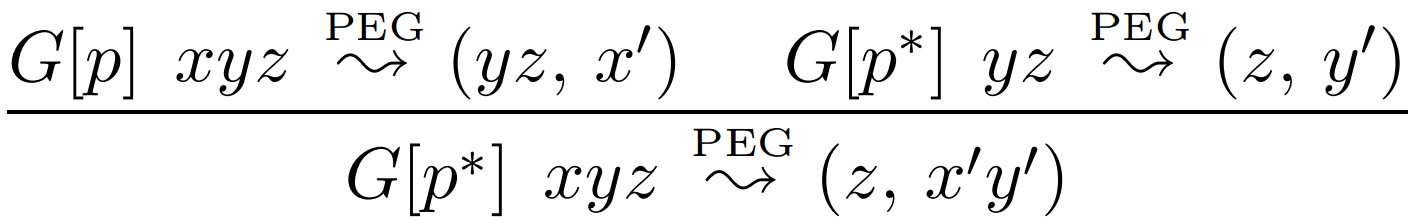
\includegraphics[width=0.7\textwidth]{pics/rep2} 
\end{center}
\end{frame}

\begin{frame}[fragile]
  \transwipe[direction=90]
  \frametitle{Ограниченная левая рекурсия}
\begin{itemize}
  \item $A^n$ имеет не более $n$ леворекурсивных вызовов $A$, $A^0$ всегда 
завершается ошибкой
\end{itemize}
$$
\begin{array}{crcl}
&E^0 & ::= & fail \\ 
&E^1 & ::= & E^0 + n / n = \bot + n / n = n \\
&E^2 & ::= & E^1 + n / n = n + n / n \\
&E^3 & ::= & E^2 + n / n = (n + n / n) + n / n\\
& & \dots &  \\
&E^n & ::= & E^{n-1} + n / n \\
\end{array}
$$ 
\end{frame}

\begin{frame}[fragile]
  \transwipe[direction=90]
  \frametitle{Борьба с левой рекурсией}
\begin{itemize}
  \item Ищем значение $n$ для каждого леворекурсивного нетерминала
  \item Подбирается такая граница, чтобы префикс, обработанный правилом, имел 
максимальную длину
  \item Промежуточные значения сохраняются в табличку $L$
  \begin{itemize}
    \item $L[(A, x) \rightarrow X](B, y) = L(B, y)$, если $B \neq A$ или $y 
\neq x$
    \item $L[(A, x) \rightarrow X](A, x) = X$
  \end{itemize}
\end{itemize}
\end{frame}

\begin{frame}[fragile]
  \transwipe[direction=90]
  \frametitle{Обработка леворекурсивного нетерминала}
\begin{center}
  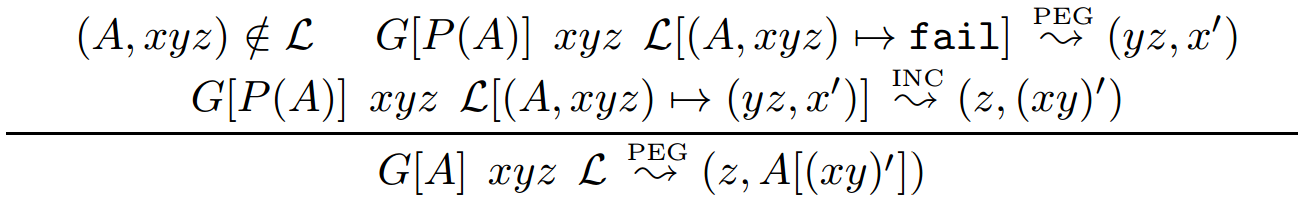
\includegraphics[width=1.0\textwidth]{pics/lvar1}  \\~\\     \pause
  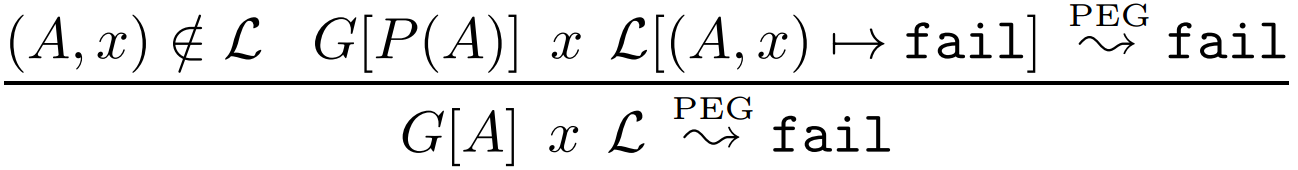
\includegraphics[width=0.7\textwidth]{pics/lvar2}  \\~\\     \pause 
  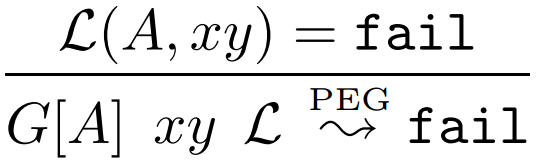
\includegraphics[width=0.3\textwidth]{pics/lvar3}  \\~\\     \pause
  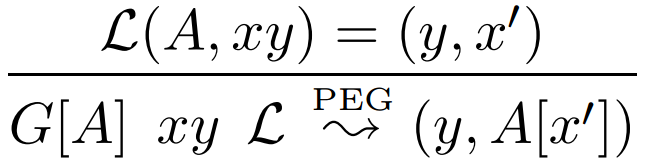
\includegraphics[width=0.35\textwidth]{pics/lvar4}  
\end{center}
\end{frame}

\begin{frame}[fragile]
  \transwipe[direction=90]
  \frametitle{Семантика отношения INC}
\begin{center}
  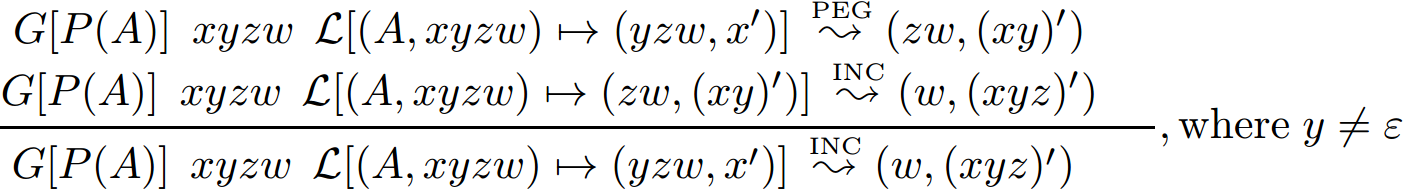
\includegraphics[width=1.0\textwidth]{pics/incr1}  \\~\\     \pause
  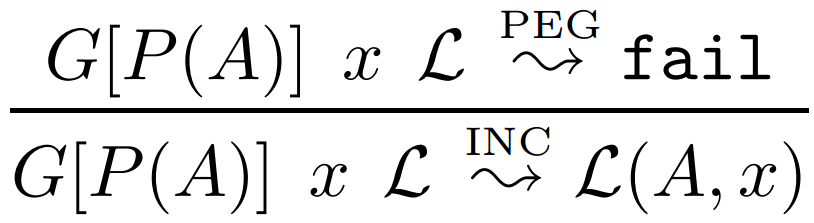
\includegraphics[width=0.3\textwidth]{pics/incr2}  \\~\\     \pause
  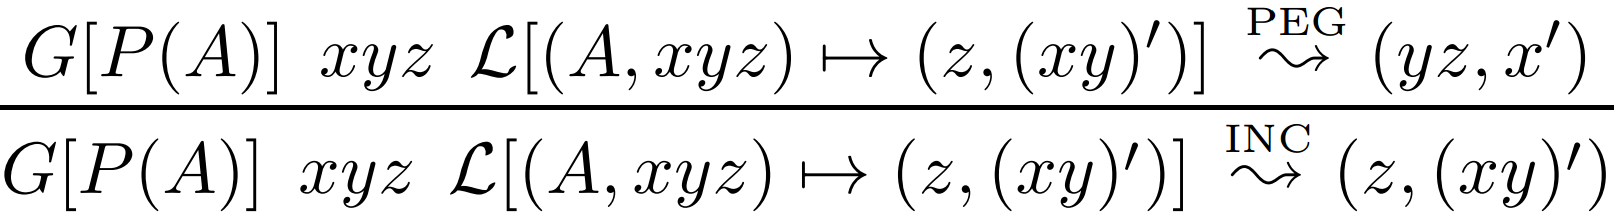
\includegraphics[width=0.7\textwidth]{pics/incr3}  
\end{center}
\end{frame}



\begin{frame}[fragile]
  \transwipe[direction=90]
  \frametitle{Литература}
\begin{itemize}
  \item Left recursion in Parsing Expression Grammars: \url{http://arxiv.org/pdf/1207.0443.pdf}
\end{itemize}

\end{frame}
\end{document}
